\documentclass[12pt,a4paper]{article}
\usepackage[utf8]{inputenc}
\usepackage[T2A]{fontenc}
\usepackage[russian,english]{babel}
\usepackage{amsmath}
\usepackage{amsfonts}
\usepackage{amssymb}
\usepackage{graphicx}
\usepackage[left=2cm,right=2cm,top=2cm,bottom=2cm]{geometry}
\usepackage{calc}
\usepackage{setspace}
\usepackage{indentfirst}
\usepackage{caption}
\usepackage{xcolor}


\title{
    Отчет о выполнении лабораторной работы 3565.32.50494452
    
    Оценка эффективности SIMD-оптимизаций программы Mandelbrat2
    }
    
\author{Швабра Владимир Сергеевич, Б01-411}

\captionsetup[figure]{name=Рис.}

\begin{document}
\maketitle

\newpage

\section{Аннотация}
\subsection{Цели работы}  
\begin{enumerate}
    \item Научиться применять различные низкоуровневые оптимизации на примере расчёта множества Мандельброта.
    \item Научиться оценивать эффективность работы программы
\end{enumerate}

\subsection{Теоретическая справка}

Сначала рассмотрим базовую последовательную модель выполнения инструкций (SEQ), а затем перейдем к современным конвейерным реализациям (PIPE) с предсказанием переходов.

\subsubsection{Последовательная модель выполнения (SEQ)}
На рисунке \ref{fig:seq} представлена последовательная модель обработки инструкций:

\begin{figure}[h!]
\centering
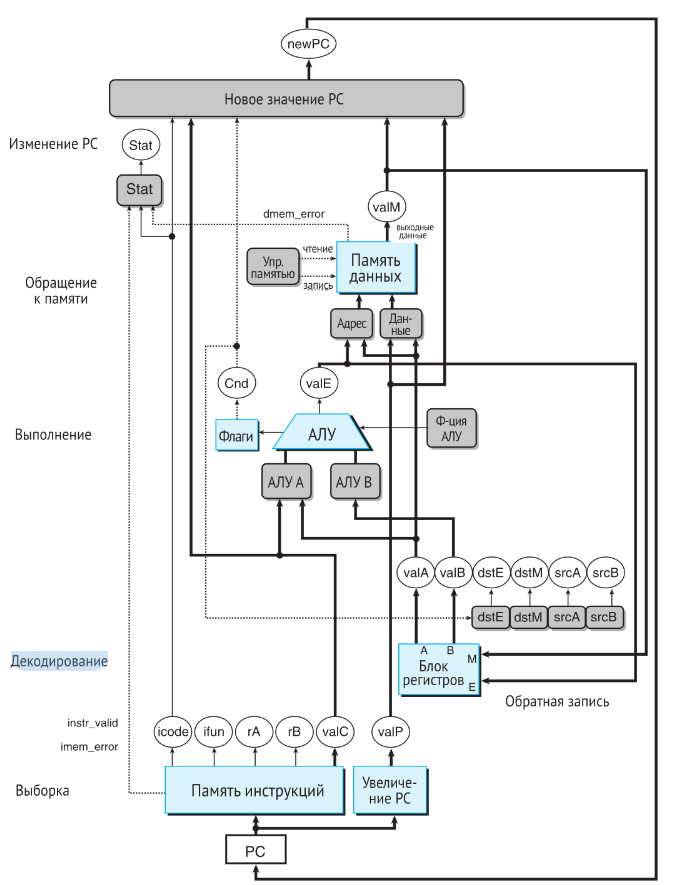
\includegraphics[width=0.9\textwidth]{seq.png}
\caption{Блок-схема последовательной обработки инструкций (SEQ)}
\label{fig:seq}
\end{figure}

\paragraph{Этапы последовательной обработки}

\begin{enumerate}
    \item \textbf{Выгрузка (F)}:
    \begin{itemize}
        \item Извлекает инструкцию из памяти по адресу, указанному в Program Counter (PC)
        \item Используется \textit{кэш инструкций} для ускорения доступа
        \item PC увеличивается на размер инструкции (или изменяется для инструкций перехода)
    \end{itemize}

    \item \textbf{Декодирование (D)}:
    \begin{itemize}
        \item Определяется \textit{тип операции} (арифметическая, логическая, перехода и т.д.)
        \item Выявляются \textit{операнды} (регистры, непосредственные значения, адреса памяти)
        \item Для операций с памятью вычисляются эффективные адреса
        \item Подготавливаются сигналы управления для следующих этапов
    \end{itemize}

    \item \textbf{Выполнение (E)}:
    \begin{itemize}
        \item Выполнение арифметических или логических операций в \textit{АЛУ} (Арифметико-Логическом Устройстве)
        \item Для условных переходов - проверка условий и вычисление адреса перехода
    \end{itemize}

    \item \textbf{Обращение к памяти (M)}:
    
    Этот этап присутствует только для инструкций работы с памятью.
    \begin{itemize}
    \item Для загрузки: чтение данных из памяти по вычисленному адресу
    \item Для записи: запись данных в память по вычисленному адресу
    \item Используется \textit{кэш данных} для ускорения доступа
    \item Обработка кэш-промахов и обращение к основной памяти при необходимости
    \end{itemize}

    \item  \textbf{Обратная запись (W)}:
    \begin{itemize}
        \item Для арифметических операций - запись в регистр-приемник
        \item Для операций загрузки - запись данных из памяти в регистр
    \end{itemize}

    \item \textbf{Изменение PC}:
    \begin{itemize}
        \item Для обычных инструкций: PC уже был увеличен на этапе выгрузки
        \item Для инструкций перехода: PC изменяется на новое значение
        \item Для условных переходов: PC изменяется только если условие истинно
        \item Обработка исключений и прерываний также может изменить PC
    \end{itemize}
\end{enumerate}

\paragraph{Ограничения SEQ}
Главный недостаток последовательной модели — низкая эффективность. Каждый этап задействует только часть аппаратных ресурсов процессора, остальные простаивают.

\subsection{Конвейерная модель выполнения (PIPE)}
Современные процессоры используют конвейерную обработку, как показано на рисунке \ref{fig:pipe}.

\begin{figure}[h!]
\centering
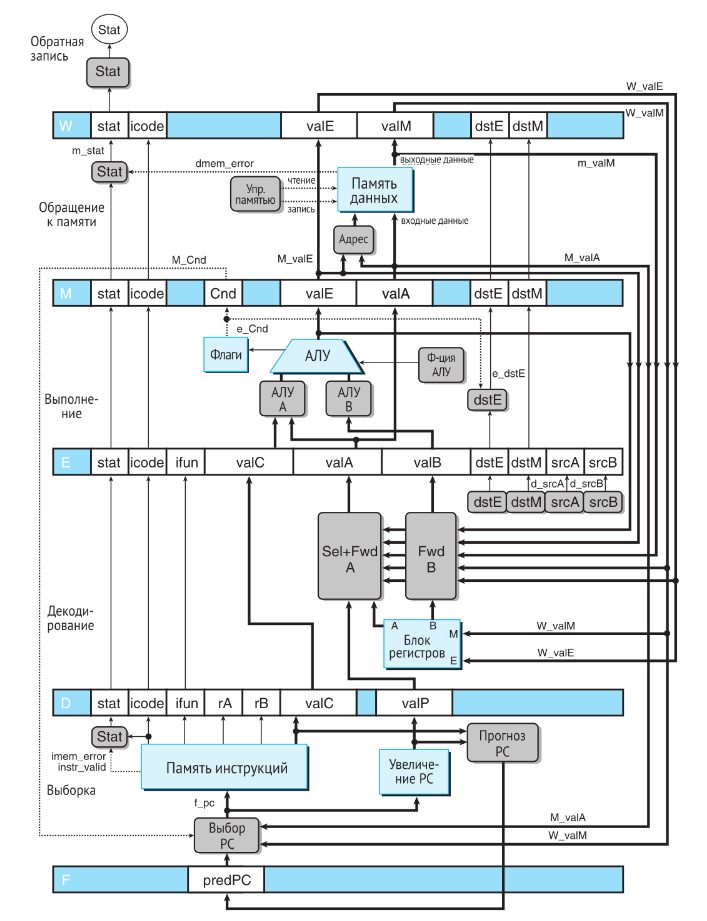
\includegraphics[width=0.8\textwidth]{pipe.png}
\caption{Блок-схема конвейерной обработки инструкций (PIPE)}
\label{fig:pipe}
\end{figure}

Из общих изменений в схеме добавились конвейерные регистры между каждой соседней парой этапов обработки инструкций. Это сделано для возможности выполнения разных этапов разных инструкций параллельно, как показно на рисунке \ref{fig:pipeline}.

\begin{figure}[h!]
    \centering
    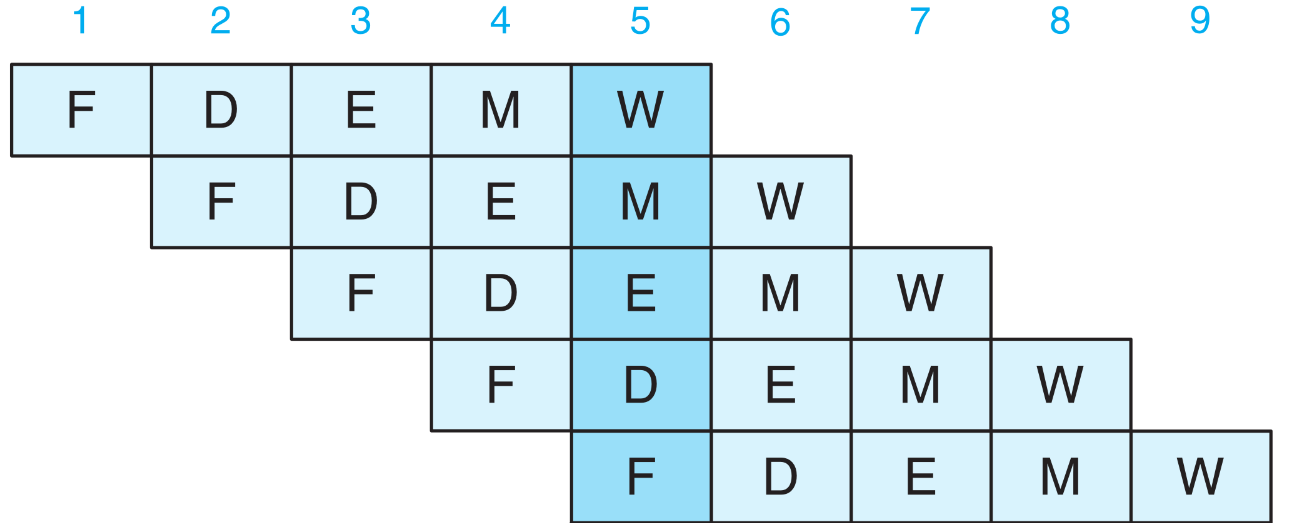
\includegraphics[width=0.8\textwidth]{pipeline.png}
    \caption{Визуализация конвейерной обработки инструкций}
    \label{fig:pipeline}
\end{figure}

\subsubsection{Предсказание РС}

Если обрабатываемая инструкция не является условным переходом, то мы можем однозначно определить следующее значение PC, но иначе нет.

\begin{itemize}
    \item \textbf{Инструкции не выполняющие "прыжок" - } так как мы знаем размер каждой инструкции, то можем прибавить его к PC.
    \item \textbf{CALL, JMP, RET - } мы знаем адрес, на который нужно перейти \textit{в любом} случае.
    \item \textbf{Условный переход - } До проверки условия мы не знаем куда надо делать "прыжок".
\end{itemize}

Проблему с условными переходами можно решить приостановкой загрузки новых инструкций в конвейер до момента вычисления условия, но есть решение лучше. Мы попробуем угадать произойдёт переход или нет и продолжать подгружать операции с соответствующего места, а в случае ошибочного предсказания сбросить загруженные инструкции, что, конечно, ударит по производительности.

Существует много различных стратегий для предсказания переходов, но мы не будем в это углубляться. Отметим лишь, что для облегчения работы предсказателю, не стоит писать сложных условий без необходимости. Также нужно знать об операциях условного перемещения, которые могут улучшить производительность ветвлений.

\subsubsection{Риски по данным}

Но схема на рисунке \ref{fig:pipeline} будет работать корректно только если во всех инструкциях, которые выполняются параллельно не будет \textit{зависимости по данным}, что может часто не соблюдаться. Приведём методы разрешения таких зависимостей.

\begin{itemize}
    \item \textbf{NOP:} самое лёгкое решение. На этапе генерации ассемблера проставить пустые инструкции в количестве необходимом, для такого чтобы устранить параллельное выполнение инструкций зависимых по данным (Рис. \ref{fig:nop}).
    \begin{figure}[h!]
        \centering
        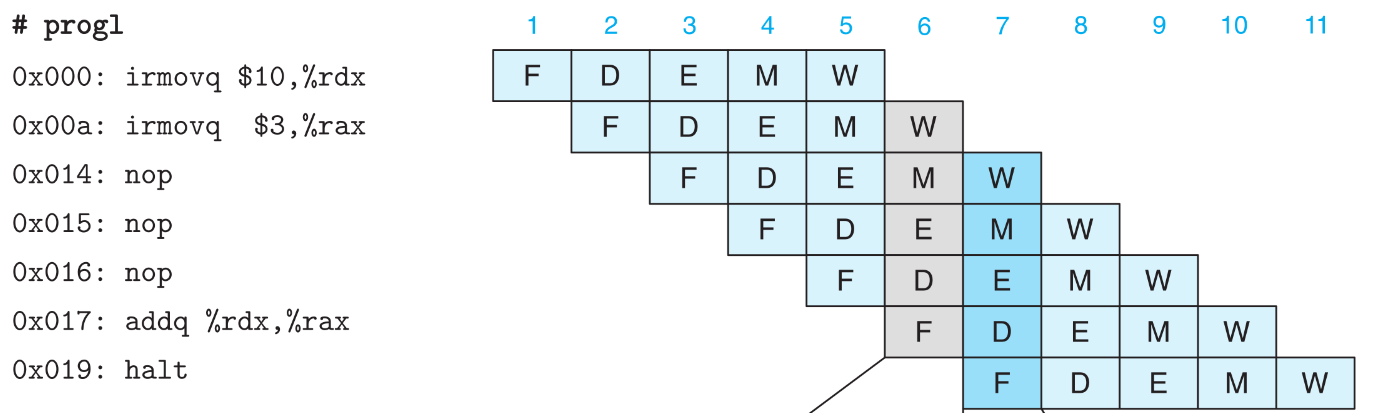
\includegraphics[width=0.8\textwidth]{nop.png}
        \caption{Останова, реализованная через NOP для решения проблемы риска по данным}
        \label{fig:nop}
    \end{figure}

    \item \textbf{"Пузырёк" (Привет дед!): } Аппаратная приостановка конкретных этапов обработки инструкций, зависящих по данным (Рис. \ref{fig:babble}).
    \begin{figure}[h!]
        \centering
        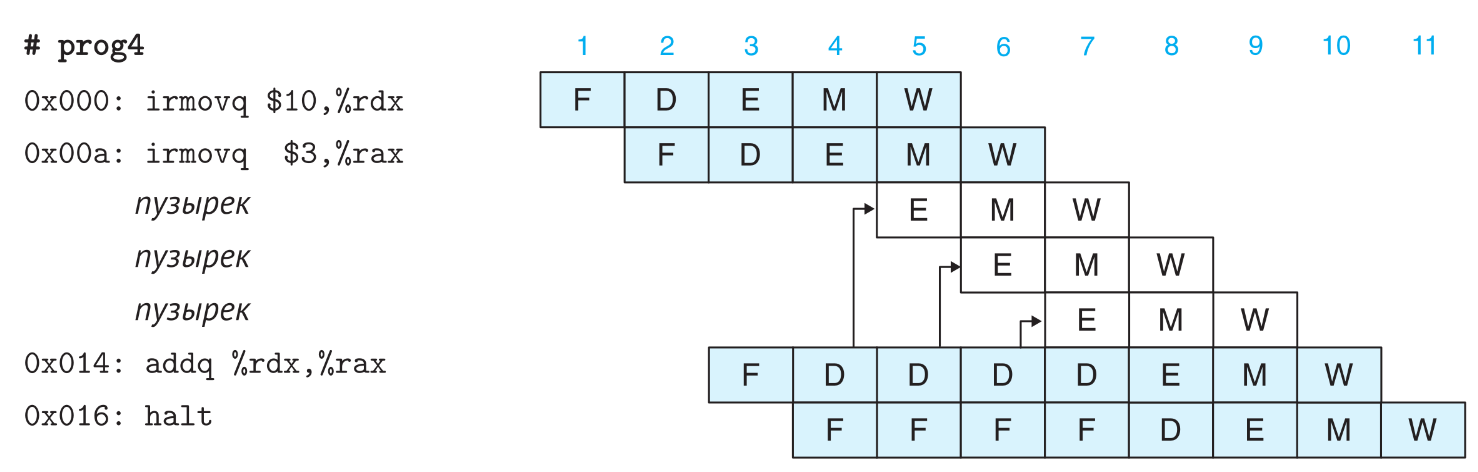
\includegraphics[width=0.8\textwidth]{babble.png}
        \caption{Останова, реализованная через "пузырёк" для решения проблемы риска по данным}
        \label{fig:babble}
    \end{figure}

    \item \textbf{Продвижение: } Мы добавляем в нашу конструкцию процессора (Рис. \ref{fig:pipe}) возможность передачи значений (регистров, либо памяти) в предыдущие этапы обработки инструкций, чтобы ожидающая инструкция могла использовать уже вычисленное значение до окончания обработки ожидаемой инструкции.
\end{itemize}

\subsubsection{Взаимосвязь функциональных блоков}

В настоящих процессорах, очевидно, есть несколько функциональных блоков, каждый из которых занимается обработкой операций того или иного типа. Это позволяет выполнять некоторые операции не по порядку. Такая архитектура процессора называется суперскалярной (Рис \ref{fig:superscalar}) и хорошо дополняет конвейерное устройство функциональных блоков.

Распределением инструкций по функциональным блокам занимается \textit{блок управления инструкциями (БУИ (это я ввёл сам, так не называют, просто чтобы меньше писать (лисп сосать (дед упрлс (а стоп, это же не гайд на летку (ну ладно, пока (швабра)))))))}. В частности на всех современных процессорах есть блок для обработки ветвлений, который пытается предсказать условные переходы (аналогично предсказателю PC в рамках одного конвейера, но на уровень выше). Такая организация обработки инструкций называется \textit{спекулятивным выполнением}.

\begin{figure}[h!]
    \centering
    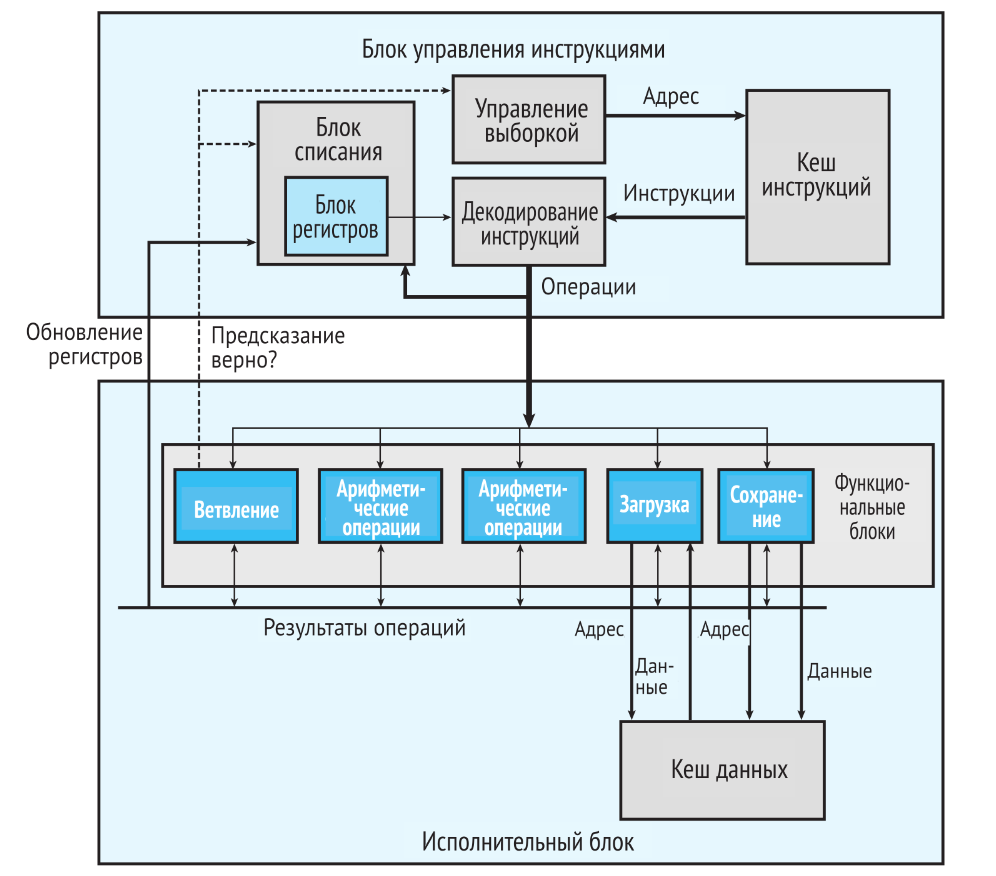
\includegraphics[width=0.8\textwidth]{supscalar.png}
    \caption{Блок-схема суперскалярного процессора}
    \label{fig:superscalar}
\end{figure}


\subsection{Оптимизации}

На основе знаний изложенных выше мы можем "класть" наш код на аппаратуру применением низкоуровневых оптимизаций, чтобы увеличить производительность. Некоторые из них мы сейчас опишем


\subsubsection{Вынос кода}

Если в цикле вычисляется значение переменной и не меняется на всех итерациях цикла, то для данного значения стоит завести константу вне цикла и использовать её. Аналогично можно поступить при постоянном обращении к памяти, правда это будет эффективно в случае, если есть свободные регистры для сохранения переменной.

\newpage

\paragraph{Пример}
\begin{verbatim}
// До оптимизации
for (size_t i = 0; i < n; ++i) {
    double result = sin(x) * arr[y] + i;  // sin(x) и arr[y] не зависят от i
    printf("%f\n", result);
}

// После оптимизации
double sin_x = sin(x);
double arr_y = arr[y];
for (size_t i = 0; i < n; ++i) {
    double result = sin_x * arr_y + i;
    printf("%f\n", result);
}
\end{verbatim}

\subsubsection{Уменьшение рисков по данным}

Стоит уметь представлять в голове как конвейерная и суперскалярная архитектура будут обрабатывать инструкции и минимизировать простои процессора. Допустим, если есть возможность переставить вычисление независимых операций, то их можно поставить между зависимыми, чтобы занять неиспользуемое время.

\newpage

\paragraph{Пример}
\begin{verbatim}
// До оптимизации
float x = y * z;  // Независимая операция
float a = b * c;
float d = a + e;  // Зависит от a

// После оптимизации
float a = b * c;
float x = y * z;   // Независимая операция
float d = a + e;
\end{verbatim}

\subsubsection{Комбинация развёртывания цикла и аккумулятора}
\indent

\textbf{Развёртывание: } это преобразование программы, которое уменьшает количество итераций за счет увеличения количества вычислений в каж­дой итерации. Развертывание цикла может улучшить производительность по двум причинам. Во-первых, уменьшается количество операций, не влияющих непосредственно на результат программы, таких как вычисление индекса и условное ветвление. Во-вторых, открываются возможности для дальнейшего преобразования кода при помощи аккумуляторов.

\textbf{Аккумуляторы: } Для ассоциативной и коммутативной комбинирующей операции (например для целочисленного сложения или умножения) производительность можно повысить, разбив набор комбинирующих операций на две или более частей, и комбинировать их результаты в конце. 

Без учёта накладных расходов использование описанных подходов можно увеличить скорость выполнения цикла во столько раз, на сколько порядков проведено развёртывание. Конечно, это можно делать не бесконечно, ведь в какой-то момент регистров для аккумуляторов не будет хватать и они будут сохраняться в переменные, что только замедлит обработку инструкций. Подробную оценку производительности читайте в БХ (байт для будущих пекусов).

\paragraph{Пример}
\begin{verbatim}
// До оптимизации
float sum = 0;
for (int i = 0; i < n; i++) {
    sum += array[i];
}

// После оптимизации (развёртывание 4x + аккумуляторы)
float sum0 = 0, sum1 = 0, sum2 = 0, sum3 = 0;
for (int i = 0; i < n; i += 4) {
    sum0 += array[i];
    sum1 += array[i+1];
    sum2 += array[i+2];
    sum3 += array[i+3];
}
float sum = sum0 + sum1 + sum2 + sum3;
\end{verbatim}

\subsubsection{Применение векторных инструкций (SIMD)}

Модель выполнения инструкций SIMD позволяет производить одну операцию сразу с несколькими данными в соответствующих функциональных блоках с поддержкой векторных операций. Использование таких инструкций очень хорошо сочетается с вышеперечисленными оптимизациями. 

\paragraph{Пример}
\begin{verbatim}
#include <immintrin.h>

// До оптимизации
for (int i = 0; i < n; i++) {
    c[i] = a[i] + b[i];
}

// После оптимизации
for (int i = 0; i < n; i += 4) {
    __m128 va = _mm_load_ps(&a[i]);
    __m128 vb = _mm_load_ps(&b[i]);
    __m128 vc = _mm_add_ps(va, vb);
    _mm_store_ps(&c[i], vc);
}
\end{verbatim}

\end{document}